%\section{Signal region, control region and validation region definitions}
In this analysis,  three different regions are considered, refering to specific areas in the kinematic phase space of the collected events (see Figure \ref{fig:stat:regions}).\\
\textbf{\acp{SR}} are regions in phase space showing the largest possible contributions of the \ac{BSM} signal searched for and the most promising differentiation between the signal and \ac{SM} background.  In this regions,  a \textit{blinded analysis approach} is followed.  Until all background estimations in the signal region with their associated systematic uncertainties are finalised,  no comparison of data to the background or signal expectation can be performed.  \\
%This is in order to avoid any bias in the data-driven estimation of \ac{SM} backgrounds.
\textbf{\acp{CR}} are used to estimate the backgrounds in the signal region by comparing the prediction of background processes with the data observed in the said region.
They are designed to be enriched with one specific background.  Details about the way in which backgrounds in the \acs{SR}s are estimated are given later in this chapter. Control Regions are orthogonal to signal regions to make a statistically independent measurement of the background normalisation.  \\
\textbf{\acp{VR}} are defined in combination with control regions in order to validate the extrapolation from \acs{CR} to \acs{SR}.

%One concept used throughout this thesis to evaluate different background processes and particularly the agreement of its modelling in simulation with the observed data is the concept on control and validation regions.  
%Control regions are regions in kinematic phase space of the collected events that are enriched in one \ac{SM} process. These control regions are used to compare the prediction of background processes with the data observed in the region. 
\begin{figure}
\centering
		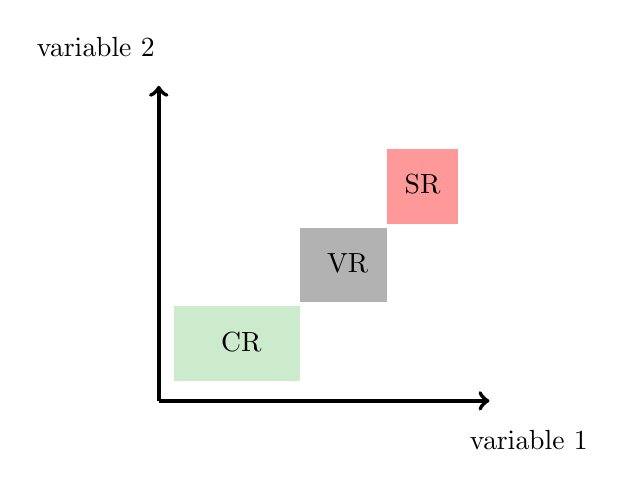
\begin{tikzpicture}
		\draw[line width =1.5pt,->] (0,0) -- (4.2,0);
		\node[](A) at (4.7,-0.5) {variable 1};
		\draw[line width =1.5pt,->] (0,0) -- (0,4.0);
		\node[](B) at (-0.8,4.5) {variable 2};
		\fill[green!60!black!20] (0.2,0.25) rectangle (1.8,1.2);
		\node[](E) at (1.05,0.75) {CR};
		\fill[gray!60] (1.8,1.25) rectangle (2.9,2.2);
%				\fill[gray!60] (1.8,1.25) rectangle (2.9,2.2);
		\node[](L) at (2.4,1.75) {VR};
		\fill[red!40] (2.9,2.25) rectangle (3.8,3.2);
		\node[](M) at (3.35,2.75) {SR};
		\end{tikzpicture}
		\caption{Visualisation of signal, control and validation regions and a typical arrangement in phase space \label{fig:stat:regions}}
\end{figure}

